\documentclass[12pt,a4paper]{article}

\usepackage[utf8]{inputenc}
\usepackage[T1]{fontenc}
\usepackage[danish]{babel}
\usepackage{geometry}
\usepackage{enumitem}
\usepackage{parskip}
\usepackage{booktabs}
\usepackage{array}
\usepackage{longtable}
\usepackage{hyperref}
\usepackage{tikz}

\geometry{margin=2.5cm}

\newcommand{\appname}{Nemlig.com (desktop)}

\title{opgave i Interaktionsdesign\\[0.5em]
       \large \appname}
\author{Silas Benjamin Steen Andersen}
\date{27.\ marts 2026}

% =========================================================
\begin{document}
\maketitle
\vspace{0.5em}
\noindent
\textbf{Valgt applikation:} \appname\\
\textbf{Afleveringsdato:} Fredag 27. marts 2026 kl. 16:00

\newpage

% =========================================================
\section*{Spørgsmål 1: Brugere, opgaver og vigtige aspekter}

Jeg har valgt at tage udgangspunkt i \textbf{Nemlig.com (Computer)}, et dansk online supermarked
hvor brugeren kan udvælge dagligvarer og bestille levering til døren. I det følgende beskriver
jeg mine antagelser om brugere, opgaver og kontekst. Antagelserne er ikke baseret på egen
empirisk undersøgelse, men er et udgangspunkt, der i praksis bør afprøves og raffineres gennem
user research (jf.\ Hornbæk et al., 2025, kap.\ 10).

\subsection*{(a) Antagelser om brugere, opgaver og brugskontekst}
Jeg beskriver målgruppen gennem kriterier for \textit{adfærd},
\textit{teknologibrug} og \textit{demografi} (jf.\ Hornbæk et al., 2025, kap.\ 10).


\textbf{Målgruppeprofil 1: ``Den travle børnefamilie''}
\begin{itemize}[leftmargin=*,itemsep=0.2em]
  \item \textbf{Adfærd (behavioral):} Handler dagligvarer 1--2 gange ugentligt, vil minimere
        tid brugt på planlægning og indkøb, og prioriterer en stabil/forudsigelig levering.
        Bruger ofte ``genkøb''/rutiner frem for at udforske nye varer.
  \item \textbf{Teknologibrug (technological):} Har høj rutine i webshopping (fx andre
        webshops), bruger pris-/tilbudsfiltre og forventer hurtig søgning, tydelig feedback og
        let redigering af kurv.
  \item \textbf{Demografi (demographical):} To voksne, mindst ét barn, mellem-høj
        husstandsindkomst, bor i område hvor levering er tilgængelig.
\end{itemize}

\textbf{Målgruppeprofil 2: ``Tilbudsjægeren''}
\begin{itemize}[leftmargin=*,itemsep=0.2em]
  \item \textbf{Adfærd:} Sammenligner priser/tilbud, skifter mellem mærker og størrelser, og
        bruger tid på at optimere kurven.
  \item \textbf{Teknologibrug:} Komfortabel med filtre/sortering og mange faner; kan blive
        påvirket af interface-elementer der fremhæver bestemte valg (fx ``mest populære'' eller
        premium-alternativer).
  \item \textbf{Demografi:} Kan være studerende eller husstand med stramt budget; geografisk
        variation.
\end{itemize}

\textbf{Typiske opgaver} i Nemlig.com antages at være (1) finde specifikke varer via
søgning/kategorier, (2) lægge varer i kurv og justere mængder, (3) vælge leveringstidspunkt og
gennemføre checkout, (4) håndtere afvigelser såsom udsolgte varer/substitutioner, og
(5) \textbf{Fokusopgave (til resten af opgaven):} Brugeren søger efter tre konkrete dagligvarer
(fx ``mælk'', ``pasta'' og ``bananer'') og lægger én af hver i kurven via søgning og
produktliste på desktop.

\textbf{Brugskontekst} antages typisk at være hjemme foran computer i en hverdagssituation med
tids- og opmærksomhedspres (multitasking), hvor fejl (fx forkert vare/størrelse/levering) har
direkte konsekvenser i hverdagen.

\subsection*{(b) Tre prioriterede aspekter af usability og user experience}
På baggrund af (a) vurderer jeg følgende tre aspekter som vigtigst (prioriteret):

\begin{enumerate}[leftmargin=*,itemsep=0.3em]
  \item \textbf{Effektivitet (usability):} Brugeren skal hurtigt kunne nå fra ``jeg mangler
        varer'' til en færdig ordre. \\
        \textit{Mulig måling:} Tid på opgave, antal klik/handlinger, succesrate, samt en
        KLM-analyse for en klart afgrænset opgave. \\
        \textit{Udfordringer:} Tidsmålinger afhænger af erfaring og strategi (novice vs.\
        rutineret), og KLM forudsætter en idealiseret ``øvet'' bruger.

  \item \textbf{Fejlforebyggelse og recovery (usability):} Det skal være svært at lave fejl og
        let at opdage/rette dem (fx mængder, substitutioner, leveringsvalg og skjulte
        omkostninger). \\
        \textit{Mulig måling:} Antal fejl og rettelser, hvor ofte brugere fortryder/retter, og
        hvor hurtigt de kan rette en fejl uden at miste overblik. \\
        \textit{Udfordringer:} Hvad der tæller som en ``fejl'' kan være tvetydigt (fx om en
        substitution opleves som fejl eller acceptabelt alternativ).

  \item \textbf{Oplevet kontrol og tillid (user experience):} Brugeren skal føle sig tryg ved
        at systemet afspejler deres intentioner (hvad bestilles, hvornår leveres, og hvad koster
        det samlet). \\
        \textit{Mulig måling:} Spørgeskema-items om tillid/kontrol (fx 1--7), korte interviews
        efter opgaven, samt observation af tøven/tilbageklik som indikator på usikkerhed. \\
        \textit{Udfordringer:} UX-mål har ofte lav præcision og kan være påvirket af social
        desirability bias og kontekst (fx om brugeren allerede kan lide brandet) (jf.\ Hornbæk et al., 2025, s. 237).
\end{enumerate}

\newpage
\section*{Spørgsmål 2: Ekspertevaluering}

\subsection*{(a) Valg af metode og diskussion}

\textbf{Valgt metode: Heuristisk evaluering (Nielsen, 1994)}

Jeg har valgt heuristisk evaluering som min ekspertmetode. I heuristisk evaluering gennemgår en
evaluator systematisk et interface og bedømmer dets overensstemmelse med et sæt anerkendte
designprincipper -- de såkaldte heuristikker. Jeg anvender Nielsens 10 heuristikker, da de er
veldokumenterede og bredt anvendte i både praksis samt pensum (Hornbæk et al., 2025).\\
Metoden er velegnet til dette projekt, fordi den kan gennemføres af én
evaluator uden brug af testdeltagere, kræver begrænset planlægningstid og giver konkrete og handlingsorrienteret fund. Da opgaven har en stram tidsramme og fokuserer på et klart afgrænset
flow (søg efter- og læg vare i kurv), matcher metodens effektivitet godt.

\textbf{Fordele og ulemper sammenlignet med andre metoder:}
\begin{itemize}[leftmargin=*,itemsep=0.3em]
  \item \textit{Brugertest (tænke-højt):} Brugertest afslører reelle brugsvanskeligheder og
        uventede adfærdsmønstre, som en ekspert kan overse. Til gengæld kræver det rekruttering,
        mere tid og ekspertise i facilitering. Heuristisk evaluering er hurtigere, men risikerer
        at misse kontekstspecifikke problemer (som fx. kognitiv overbelastning hos en travl
        børnefamilie).
  \item \textit{Cognitive walkthrough:} Denne metode analyserer ligesom heuristisk evaluering
        opgaveflow uden brugere, men fokuserer specifikt på lærbarhed og den nye brugers
        forklaringsmodel (jf.\ Hornbæk et al., 2025, s. 721). Heuristisk evaluering er bredere og bedre til at fange generelle
        designproblemer ud over lærbarhed.
  \item \textit{Spørgeskema (fx SUS):} Spørgeskemaer er hurtige at administrere og giver
        kvantitative data, men forudsætter adgang til rigtige brugere og indfanger ikke
        årsagerne til problemer.
  \item \textit{Feltstudie:} Et feltstudie giver rig kontekstuelt indblik (fx multitasking i
        hjemmet), men er meget ressourcekrævende og svær at tilrettelægge på kort tid.
\end{itemize}

Samlet set er heuristisk evaluering et godt kompromis: det er mere struktureret og reproducerbart
end uformel gennemgang, men hurtigere og billigere end brugertest. Den centrale ulempe er, at
fund ikke er valideret af rigtige brugere og i højere grad afhænger af evaluatorens vurdering.

\subsection*{(b) Planlægning og gennemførelse}

\textbf{Evalueringsopgaver:}

Evalueringen bygger på den fokusopgave, der blev defineret i Spørgsmål 1:
\begin{enumerate}[leftmargin=*,itemsep=0.2em]
  \item Søg efter ``mælk'', vælg en mælk (fx 1 liter sødmælk) og læg den i kurven.
  \item Søg efter ``pasta'', vælg én pasta og læg den i kurven.
  \item Søg efter ``bananer'', vælg én pose bananer og læg dem i kurven.
  \item Fjern én vare fra kurven.
  \item Påbegynd checkout (klik ``Gå til kurv'' og fortsæt til leveringsvalgssiden).
\end{enumerate}

\textbf{Registrering af problemer:} For hvert trin i opgaveflowet sammenholdes det observerede
interface med Nielsens 10 heuristikker. Problemer noteres med: (i) placering i flowet, (ii)
hvilken heuristik der krænkes, (iii) beskrivelse af problemet, (iv) formodet årsag og (v) en
alvorsgrad (0--4) efter Nielsens skala.

\textbf{Praktisk gennemførelse:} Evalueringen udføres ved at navigere Nemlig.com  på en standard computer. Interfacet gennemgås to gange: først
frit (orientering), derefter opgavebaseret (registrering). Alle problemer noteres løbende i et regneark og samles efterfølgende til den problemliste, der fremgår af
Bilag~A.

% ---------------------------------------------------------
\subsection*{(c) Tre konkrete udfordringer}

\begin{enumerate}[leftmargin=*,itemsep=0.4em]

  \item \textbf{Evaluatoreffekten og manglen på reelle brugerperspektiver.}
        Undervejs opdagede jeg, at det er svært at ``glemme'' sin faglige viden og forestille sig
        en normal brugers perspektiv. Jeg lagde eksempelvis straks mærke til at søgeresultaterne viste et utydeligt hierarki -- men det er uvist, om en rutineret bruger faktisk ville
        opfatte dette som et problem, eller om de blot ville ignorere de irrelevante resultater.
        Hornbæk et al.\ (2025) påpeger, at eksperter tenderer til at rapportere problemer, der
        ikke generer rigtige brugere (``false positives''), og omvendt overser problemer, der kun
        opstår i specifik brugskontekst. Udfordringen er grundlæggende: heuristisk evaluering er
        aldrig en erstatning for faktisk brugerkontakt (jf.\ Hornbæk et al., 2025, kap.\ 41).

  \item \textbf{Konsistent og retfærdig alvorsvurdering.}
        Det viste sig vanskeligt at fastsætte alvorsgrader konsistent. Et problem kan forekomme
        kritisk set fra én heuristik (fx ``æstetik og minimalistisk design''), men kun moderat
        alvorligt set fra brugerens faktiske opgave (brugeren finder alligevel sin vare trods
        støjen). Nielsens skala fra 0--4 er vejledende, men ikke algoritme\-baseret, og
        alvors\-graden vil variere fra evaluator til evaluator. Hornbæk et al.\ (2025) beskriver,
        at inter-rater-reliabilitet ved heuristisk evaluering typisk er lav, og at brug af
        multiple evaluatorer er anbefalelsesværdigt (jf.\ Hornbæk et al., 2025, s.\ 737). Da jeg er alene evaluator, er dette en
        tydelig svaghed.

  \item \textbf{Afgrænsning af hvad der udgør ét problem.}
        Flere observerede problemer overlapper hinanden eller er symptomer på den samme
        underliggende årsag (fx ``for mange elementer på produktkortet'' og ``for mange farver i
        displayet'' kan begge skyldes manglende prioritering i det visuelle hierarki). Det er
        uklart, om de skal registreres som ét problem eller flere.

\end{enumerate}

% ---------------------------------------------------------
\subsection*{(d) Opsummering af evalueringsresultater}

Evalueringen identificerede fire centrale brugbarhedsproblemer. Den fulde problemliste fremgår af Bilag~A.

De centrale fund er:

\begin{itemize}[leftmargin=*,itemsep=0.3em]
  \item \textbf{Overvældende søgeresultater (Alvorsgrad 3 -- Alvorlig):} En søgning på fx
        ``mælk'' returnerer et meget stort antal resultater uden tydelig prioritering. Brugeren
        præsenteres samtidig for reklamer og kampagnevarer imellem de organiske resultater,
        hvilket gør det svært hurtigt at identificere den ønskede vare. Dette krænker heuristik
        H8 (æstetik og minimalistisk design).

  \item \textbf{For mange trin fra ``Gå til kurv'' til faktisk kurvoversigt (Alvorsgrad 2 --
        Moderat):} Når brugeren klikker ``Gå til kurv'', mødes de af et unødvendigt antal
        mellemliggende sider og pop-ups (fx ``har du glemt disse?''-forslag) inden de ser den
        faktiske kurv. Dette strider mod H3 (brugerkontrol og -frihed) og H6 (genkendelse frem
        for hukommelse), da brugeren skal huske hvad de har lagt i kurven.

  \item \textbf{Uoverskueligt produktkort med mange farver og knapper (Alvorsgrad 3 -- Alvorlig):}
        Hvert produktkort indeholder en række handlingsknapper (tilbud, mærkeinfo, favorit,
        hurtig-tilføj m.fl.) og bruger mange og varierende baggrundsfarver til at signalere
        tilbud og kampagner. Det visuelle hierarki er svagt, og det primære handlingselement
        (``læg i kurv'') fremstår ikke tydeligt adskilt fra sekundære elementer. Dette krænker
        H8 og H4 (konsistens og standarder).

  \item \textbf{Manglende tydelig feedback ved ``lagt i kurv'' (Alvorsgrad 2 -- Moderat):}
        Når en vare lægges i kurven, er den visuelle bekræftelse lille og kortvarig. For en
        bruger, der arbejder hurtigt eller er distraheret, er det uklart om handlingen lykkedes.
        Dette krænker H1 (synlighed af systemstatus).
\end{itemize}

\newpage
% =========================================================
\section*{Spørgsmål 3: Redesign-forslag}

Redesignet tager udgangspunkt i \textbf{problem \#3 fra den heuristiske evaluering}: overfyldt produktkort med mange farver, ikoner og knapper, der skjuler den primære handling: ``Læg i kurv'' i visuel støj (H8, H4). Forslaget er et \emph{forenklet produktkort med
hover-kurv-interaktion}: kortet viser normalt kun produktbillede, navn og pris; når brugeren
fører musemarkøren over kortet, fremkommer automatisk et fremtrædende kurv-ikon centralt på
kortet som den \emph{eneste} synlige handling. Derved adresseres også delvist problem~\#4
(H1: svag feedback), idet hover-tilstanden erstatter den kortvarige animation med en tydelig
interaktiv indikation.

\subsection*{(a) Illustrationer af redesign-forslaget}

\begin{figure}[h!]
\centering
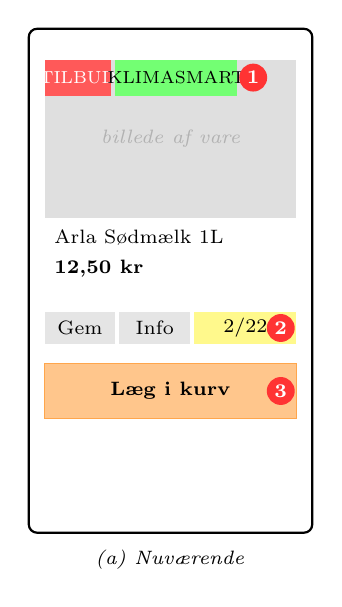
\begin{tikzpicture}[font=\scriptsize, x=1cm, y=1cm]
  % --- Nuværende produktkort ---
  \draw[rounded corners=3pt, thick] (0,0) rectangle (3.6,6.4);
  \fill[gray!25] (0.2,4.0) rectangle (3.4,6.0);
  \node[gray!60] at (1.8,5.0) {\itshape billede af vare};
  \fill[red!65]   (0.2,5.55) rectangle (1.05,6.0);
  \node[white, scale=0.9] at (0.625,5.78) {TILBUD};
  \fill[green!55] (1.1,5.55)  rectangle (2.65,6.0);
  \node[scale=0.9] at (1.875,5.78) {KLIMASMART};
  \node[anchor=west] at (0.2,3.75) {Arla S\o dm\ae lk 1L};
  \node[anchor=west] at (0.2,3.35) {\textbf{12,50 kr}};
  \fill[gray!20] (0.2,2.4) rectangle (1.1,2.8);
  \node at (0.65,2.6) {Gem};
  \fill[gray!20] (1.15,2.4) rectangle (2.05,2.8);
  \node at (1.6,2.6) {Info};
  \fill[yellow!45] (2.1,2.4) rectangle (3.4,2.8);
  \node at (2.75,2.6) {2/22};
  \fill[orange!45] (0.2,1.45) rectangle (3.4,2.15);
  \draw[orange!70]  (0.2,1.45) rectangle (3.4,2.15);
  \node at (1.8,1.8) {\textbf{L\ae g i kurv}};
  \node[circle, fill=red!80, text=white, inner sep=1.3pt] at (2.85,5.78) {\textbf{1}};
  \node[circle, fill=red!80, text=white, inner sep=1.3pt] at (3.2,2.6)   {\textbf{2}};
  \node[circle, fill=red!80, text=white, inner sep=1.3pt] at (3.2,1.8)   {\textbf{3}};
  \node[below] at (1.8,-0.1) {\textit{(a) Nuv\ae rende}};
\end{tikzpicture}%
\hspace{0.7cm}%
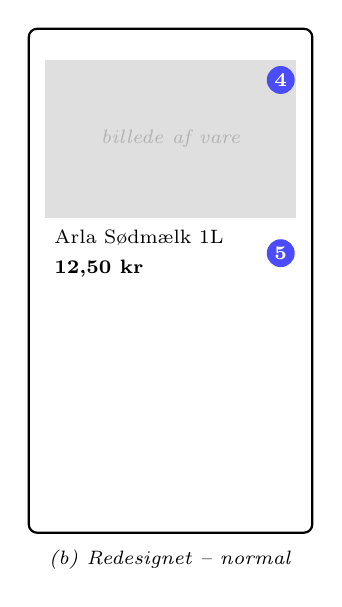
\begin{tikzpicture}[font=\scriptsize, x=1cm, y=1cm]
  % --- Redesignet: normal tilstand ---
  \draw[rounded corners=3pt, thick] (0,0) rectangle (3.6,6.4);
  \fill[gray!25] (0.2,4.0) rectangle (3.4,6.0);
  \node[gray!60] at (1.8,5.0) {\itshape billede af vare};
  \node[anchor=west] at (0.2,3.75) {Arla S\o dm\ae lk 1L};
  \node[anchor=west] at (0.2,3.35) {\textbf{12,50 kr}};
  \node[circle, fill=blue!70, text=white, inner sep=1.3pt] at (3.2,5.75) {\textbf{4}};
  \node[circle, fill=blue!70, text=white, inner sep=1.3pt] at (3.2,3.55) {\textbf{5}};
  \node[below] at (1.8,-0.1) {\textit{(b) Redesignet -- normal}};
\end{tikzpicture}%
\hspace{0.7cm}%
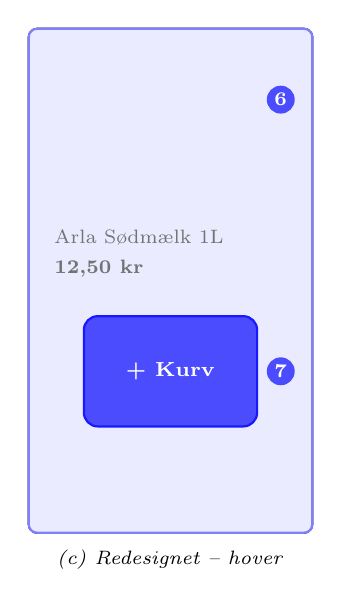
\begin{tikzpicture}[font=\scriptsize, x=1cm, y=1cm]
  % --- Redesignet: hover-tilstand ---
  \draw[rounded corners=3pt, thick] (0,0) rectangle (3.6,6.4);
  \fill[gray!20] (0.2,4.0) rectangle (3.4,6.0);
  \node[gray!55] at (1.8,5.0) {\itshape billede};
  \fill[blue!8]  (0.01,0.01) rectangle (3.59,6.39);
  \draw[blue!50, thick, rounded corners=3pt] (0,0) rectangle (3.6,6.4);
  \node[anchor=west, black!55] at (0.2,3.75) {Arla S\o dm\ae lk 1L};
  \node[anchor=west, black!55] at (0.2,3.35) {\textbf{12,50 kr}};
  \fill[blue!70, rounded corners=5pt] (0.7,1.35) rectangle (2.9,2.75);
  \draw[blue!90, thick, rounded corners=5pt] (0.7,1.35) rectangle (2.9,2.75);
  \node[white, scale=1.05] at (1.8,2.05) {\textbf{+ Kurv}};
  \node[circle, fill=blue!70, text=white, inner sep=1.3pt] at (3.2,5.5)  {\textbf{6}};
  \node[circle, fill=blue!70, text=white, inner sep=1.3pt] at (3.2,2.05) {\textbf{7}};
  \node[below] at (1.8,-0.1) {\textit{(c) Redesignet -- hover}};
\end{tikzpicture}%
\caption{Annoterede tegninger af produktkortet. \textbf{(a)}~Nuværende design.
\textbf{(b)}~Redesignet i normal tilstand. \textbf{(c)}~Redesignet i hover-tilstand.
Røde markører (1--3): identificerede problemer. Blå markører (4--7): designtiltag.}
\label{fig:prototyper}
\end{figure}

\noindent\textbf{Annotationer:}
\textbf{1}~Farverige kampagnemærker (rød, grøn) øger visuel støj (H8).
\textbf{2}~Tre sekundære knapper konkurrerer om opmærksomheden (H8/H4).
\textbf{3}~Primær ``Læg i kurv''-knap fremstår ikke visuelt fremhævet.
\textbf{4}~Forenklet kort: kun billede, navn og pris -- intet sekundært.
\textbf{5}~Klart visuelt hierarki; reducerer kognitiv overbelastning.
\textbf{6}~Hover aktiverer blå indramning som interaktivitetssignal (H1).
\textbf{7}~Fremtrædende kurv-knap vises ved musemarkørens position (Fitts' lov).

% ---------------------------------------------------------
\subsection*{(b) Begrundelse af redesign-forslaget med designprincipper}

\textbf{Hick's lov og minimalistisk design (tænkning, H8):}
Ifølge Hick's lov stiger valgreaktionstiden med antallet af valgmuligheder
(Hornbæk et al., 2025, kap.\ 8). Det nuværende produktkort præsenterer 5--7 simultane
elementer. Det redesignede kort reducerer dette til ét valg i hover-tilstanden, hvilket
direkte sænker den kognitive belastning og reaktionstiden. Dette er i overensstemmelse med
Nielsens H8 om at fjerne irrelevant information og distraherende elementer fra interfacet.

\textbf{Fitts' lov og motorisk effektivitet (perception):}
Fitts' lov forudsiger, at pegetid afhænger af målafstand og størrelse
 (Hornbæk et al., 2025, kap.\ 7). Det nuværende interface kræver
to separate pointingoperationer: én til kortet og én til den lille ``Læg i kurv''-knap.
Hover-interaktionen eliminerer den anden operation, da kurv-knappen fremkommer \emph{ved}
musemarkørens aktuelle position, ét stort let tilgængeligt mål.

\textbf{Affordance og visuel hierarki:}
Teorien om visuelle hierarkier tilsiger, at det primære interaktionselement bør dominere
visuelt (Hornbæk et al., 2025, kap.\ 14). I redesignet skjules al sekundær information i
normaltilstanden; hover-tilstanden synliggør \emph{én} tydelig handling. Kurv-knappens
blå farve, store størrelse og centrale placering udgør en klar \emph{affordance}
(Gibson, 1977; jf.\ Hornbæk et al., 2025, kap.\ 13) og dens fremtræden kommunikerer
entydigt dens funktion uden yderligere forklaring.

% ---------------------------------------------------------
\subsection*{(c) KLM-analyse}

KLM-analysen er udført for opgaven \emph{``søg efter `mælk' og læg én mælk i kurven''}
startende fra Nemlig.coms forside. Fuldstændige analysetabeller fremgår af Bilag~B
(nuværende) og Bilag~C (redesign). Opsummering af tider:

\begin{center}
\begin{tabular}{lrr}
\toprule
& \textbf{Nuværende} & \textbf{Redesign} \\
\midrule
$t_K$ (tastetryk)  & 1{,}80\,s & 1{,}80\,s \\
$t_P$ (pointing)   & 3{,}30\,s & 2{,}20\,s \\
$t_H$ (homing)     & 1{,}20\,s & 1{,}20\,s \\
$t_M$ (mentalt)    & 4{,}80\,s & 3{,}60\,s \\
$t_R$ (system)     & 0{,}50\,s & 0{,}50\,s \\
\midrule
\textbf{Total}     & \textbf{11{,}60\,s} & \textbf{9{,}30\,s} \\
\bottomrule
\end{tabular}
\end{center}

Redesignet er \textbf{2{,}30\,s hurtigere} (ca.\ 20\,\%) end den nuværende applikation.
Besparelsen stammer fra eliminering af ét M-trin ($-1{,}20$\,s: brugeren behøver ikke
lede visuelt efter ``Læg i kurv''-knappen) og ét P-trin ($-1{,}10$\,s: kurv-knappen
fremkommer ved musemarkørens aktuelle position, så der kræves ingen ekstra pegning).

% ---------------------------------------------------------
\subsection*{(d) Beskrivelse af evaluering}
For at undersøge, om KLM-analysen giver gyldige tidsforudsigelser, foreslår jeg et kontrolleret laboratorieforsøg, hvor 12–15 erfarne webshoppere udfører præcis den opgave, som KLM-modellen er baseret på.
Forsøget gennemføres med counterbalanced rækkefølge (AB/BA), så halvdelen starter med det nuværende interface, og halvdelen med det redesignede. Dette minimerer ordenseffekter og sikrer, at tidsforskelle primært skyldes "interface variations".\\

De observerede tider sammenlignes med KLM-forudsigelserne (11{,}60\,s og 9{,}30\,s). KLM betragtes som "valid", hvis observerede gennemsnit falder inden for $\pm5$\,s af forudsigelsen (jf.\Hornbæk et al., 2025, s.\ 736). 
En central trussel mod validiteten er KLMs antagelse om eksperter og fejlfri adfærd: de fleste brugere er ikke eksperter, og observerede tider vil sandsynligvis overstige prediktionerne. 

\newpage
% =========================================================
\section*{Spørgsmål 4: Deceptive patterns i Nemlig.com}

\subsection*{(a) Tre eksempler på deceptive patterns}

Gray et al.\ (2018) definerer deceptive patterns som situationer, hvor designere bruger viden
om menneskelig adfærd til at implementere vildledende funktionalitet, der ikke er i brugerens
interesse (s.\ 1). På side 4 i samme artikel opstilles 12 typer. Nedenfor beskrives tre
eksempler fra Nemlig.com og relateres til disse typer.

\textbf{Eksempel 1: ``Sneak into Basket'' (tilføjelse til kurv uden eksplicit samtykke)}

Når brugeren klikker ``Læg i kurv'' på et produkt, viderestilles de ikke direkte til kurven.
I stedet vises to mellemliggende sider: ``Vi vil lige huske dig på\ldots'' og
``Frugt og grønt til ugen'', der præsenterer yderligere produktforslag. Siderne er designet
til at ligne en naturlig del af checkout-flowet, og det primære visuelle element er en
fremtrædende ``Tilføj''-knap for ekstra varer frem for en neutral ``Fortsæt til kurv''-knap.
Brugeren skal aktivt lede efter muligheden for at springe over.

Dette er et eksempel på \emph{Sneak into Basket} (Gray et al., 2018, s.\ 4): systemet
udnytter brugerens momentum i opgaveflowet til at indsætte yderligere valg, der er designet
til at fremkalde tilføjelser snarere end at støtte brugerens oprindelige intention.

\begin{figure}[h!]
\centering
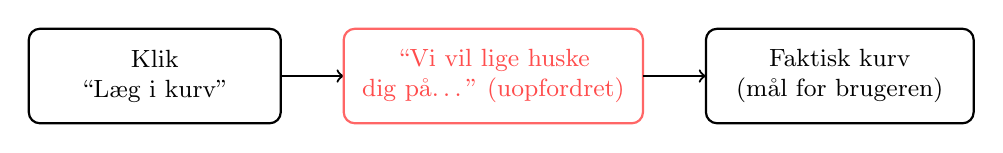
\begin{tikzpicture}[font=\small, x=1cm, y=1cm]
  % Flowdiagram: tre bokse med pile
  \draw[rounded corners=4pt, thick] (0,0) rectangle (3.2,1.2);
  \node[align=center] at (1.6,0.6) {Klik\\``Læg i kurv''};
  \draw[->, thick] (3.2,0.6) -- (4.0,0.6);
  \draw[rounded corners=4pt, thick, red!60] (4.0,0) rectangle (7.8,1.2);
  \node[align=center, red!70] at (5.9,0.6) {``Vi vil lige huske\\dig på\ldots'' (uopfordret)};
  \draw[->, thick] (7.8,0.6) -- (8.6,0.6);
  \draw[rounded corners=4pt, thick] (8.6,0) rectangle (12.0,1.2);
  \node[align=center] at (10.3,0.6) {Faktisk kurv\\(mål for brugeren)};
\end{tikzpicture}
\caption{Sneak into Basket: brugeren møder uopfordrede mersalgssider (rød boks) inden
  kurven vises.}
\label{fig:sneak}
\end{figure}

\textbf{Eksempel 2: ``Hidden Costs'' (skjulte omkostninger)}

Under browsing og produktsiden viser Nemlig.com en pris pr.\ vare, men leveringsgebyr,
servicetillæg og evt.\ pose-tillæg fremgår ikke konsekvent i produktvisningen. Disse
omkostninger dukker først op sent i checkout-processen -- på betalingssiden -- og kan samlet
beløbe sig til 30--60~kr.\ oven i den viste pris. På det tidspunkt har brugeren allerede
investeret tid og mental energi i at sammensætte kurven og vælge leveringstidspunkt, hvilket
skaber et psykologisk pres for at gennemføre købet (sunk cost).

Dette svarer til \emph{Hidden Costs} i Gray et al.\ (2018, s.\ 4): reelle omkostninger
skjules eller nedtones, indtil brugeren er dybt inde i transaktionsflowet og det er
omstændeligt at fortryde.

\textbf{Eksempel 3: ``Disguised Ad / Bait and Switch'' (skjult reklame og lokkemad)}

På Nemlig.coms forside vises en fremtrædende banner med teksten \emph{``Få 100 kr.\ til at
handle for''} med en markant knap. Designet og placeringen signalerer, at dette er en simpel
bonus, der aktiveres med ét klik -- som en rabatkode. Klikker brugeren på knappen, ledes de
imidlertid til en side, der kræver oprettelse af et abonnement (Nemlig.com~Plus) for at
modtage beløbet.

Dette kombinerer \emph{Bait and Switch} og \emph{Disguised Ad} fra Gray et al.\ (2018, s.\
4): tilbuddet lokker med en attraktiv fordel (100~kr.), men fører til et produkt/en forpligtelse
(abonnement), brugeren ikke forventede. Den reklamelignende banner er designet til at se ud
som et neutralt tilbud, ikke som en betalt/kommerciel opfordring til tilmelding.

\subsection*{(b) Konsekvenser for brugerne}

De tre deceptive patterns er direkte skadelige for de kvaliteter, der i Spørgsmål~1(b) blev
prioriteret som vigtigst: \emph{effektivitet}, \emph{fejlforebyggelse og recovery} samt
\emph{oplevet kontrol og tillid}.

\textit{Effektivitet:} Sneak into Basket tvinger brugeren igennem op til to ekstra sider ved
hvert varetilføj. For en travl børnefamilie, der har en stor indkøbsliste, ganger dette sig
hurtigt op til en markant forøgelse af samlet tid på opgaven -- præcis det aspekt, der var
højest prioriteret i Spørgsmål~1(b).

\textit{Fejlforebyggelse og recovery:} Hidden Costs skader brugerens mulighed for at sammenligne
og vurdere reelle omkostninger tidligt i processen. Fejlen (at have undervurderet totalprisen)
opdages meget sent, og recovery kræver at afbryde et næsten-fuldført køb og starte forfra --
en høj pris for den information, der burde have fremgået fra starten.

\textit{Oplevet kontrol og tillid:} Alle tre patterns underminerer brugerens oplevelse af
kontrol. Gray et al.\ (2018) understreger, at deceptive patterns netop udnytter ``the desires
of end users'' (s.\ 1) -- altså bruger kendskab til brugerens mål (spare penge, handle
effektivt) mod dem. For brugere, der opdager mønstrene, er det sandsynligt, at tilliden til
Nemlig.com som platform reduceres, hvilket på sigt kan føre til churn. For brugere, der ikke
opdager dem, sker der en usynlig overflytning af værdi fra bruger til platform (gennem mersalg,
uventede gebyrer og abonnementer), uden informeret samtykke -- hvilket udgør et etisk problem
ud over en blot designfejl.

\subsection*{(c) Sammenligning: adfærdsændring og deceptive patterns}

Lærebogen (Hornbæk et al., 2025) beskriver \emph{persuasive technology} og teknikker til
adfærdsændring som bl.a.\ \emph{nudging}, sociale normer, feedback-sløjfer og tilpasning af
standardvalg (defaults). Disse teknikker bruges til at understøtte brugerens egne mål og
til at fremme ønsket adfærd -- fx mere sund kost, fysisk aktivitet eller energibesparelse.

\textbf{Lighed:} Både persuasive design og deceptive patterns bygger på den samme
psykologiske viden om menneskelig adfærd, herunder status quo-bias, framing-effekter og
sunk cost-effekten. Et eksempel er brugen af \emph{defaults}: persuasive design kan sætte
``grøn levering'' som standard leveringsform (et miljøvenligt nudge til gavn for brugeren og
samfundet), mens deceptive patterns kan sætte et betalt nyhedsbrev som standard ved tilmelding
(til gavn for platformen). Mekanismen er identisk; intentionen og konsekvensen er modsatrettede.

\textbf{Forskel:} Den afgørende forskel er brugerens interesse. Hornbæk et al.\ (2025)
beskriver adfærdsændringsteknikker som legitime, når de \emph{støtter} brugerens egne erklærede
mål og giver brugeren en reel mulighed for at afvise eller ændre dem (autonomibevarelse).
Gray et al.\ (2018) definerer netop deceptive patterns ud fra, at de \emph{ikke} er i
brugerens interesse (s.\ 1). Hidden Costs er et konkret eksempel på, at teknikkerne adskiller
sig: et ægte nudge ville fremhæve alle omkostninger tidligt for at understøtte en informeret
beslutning; Hidden Costs skjuler dem bevidst for at reducere fravalg -- det modsatte af
informeret autonomi.

\subsection*{(d) Refleksion: at blive bedt om at anvende deceptive patterns som udvikler}

Hvis jeg som udvikler blev bedt om at implementere deceptive patterns, ville jeg opleve et
klart etisk dilemma. Gray et al.\ (2018) viser, at designere, der implementerer sådanne
mønstre, aktivt bruger deres faglige viden til at skade brugerne -- det er ikke en neutral
designbeslutning, men et informeret valg om at handle i platformens snarere end brugerens
interesse (s.\ 1).

Fra lærebogen ved jeg, at design er en praksis med reelle konsekvenser for menneskers
handlemuligheder og velvære (Hornbæk et al., 2025). Persuasive technology er kun etisk
forsvarlig, når det respekterer brugerautonomi og understøtter brugerens egne mål (Hornbæk
et al., 2025, kap.\ 19). Et krav om at anvende Hidden Costs eller Sneak into Basket er i
direkte modstrid med dette princip.

I praksis ville jeg gøre følgende:
\begin{enumerate}[leftmargin=*,itemsep=0.2em]
  \item \textbf{Undersøge intentionen:} Forespørgslen kan stamme fra forretningsmæssigt pres
        snarere end bevidst ond vilje. Jeg ville forklare, hvad deceptive patterns er, og
        dokumentere de langsigtede risici: tab af brugertillid, juridiske risici (bl.a.\ GDPR
        og EU-forbrugerbeskyttelsesregler) og omdømmeskade.
  \item \textbf{Foreslå alternativer:} I stedet for Hidden Costs ville jeg foreslå tydelig
        pris\-visning med gebyrer fremhævet tidligt -- dette \emph{øger} konverteringen hos
        brugere, der alligevel vil købe, og reducerer frustration og returns. I stedet for
        Sneak into Basket ville jeg foreslå opt-in mersalg med én tydelig ``Nej tak''-knap.
  \item \textbf{Sætte en grænse:} Hvis virksomheden fastholdt kravet om at vildlede brugerne
        efter en informeret diskussion, ville jeg nægte at implementere det og om nødvendigt
        eskalere til en faglig eller juridisk instans. Hornbæk et al.\ (2025) understreger, at
        designere har et medansvar for de systemer, de er med til at skabe -- ansvaret ophører
        ikke, fordi beslutningen tages ``et andet sted i organisationen''.
\end{enumerate}

Sammenfattende: deceptive patterns er ikke blot et designproblem, men et etisk problem, og
som (fremtidig) professionel designer anser jeg det som en kernekompetence at kunne
identificere, afvise og erstatte dem med ansvarlige alternativer.

\newpage
% =========================================================
\appendix
\section*{Bilag A: Problemliste fra heuristisk evaluering af Nemlig.com}

\noindent\textbf{Interface:} Nemlig.com (desktop, Chrome). \textbf{Dato:} 25.\ marts 2026.\\
\textbf{Evalueringsmetode:} Heuristisk evaluering (Nielsens 10 heuristikker).\\
\textbf{Alvorsgrad:} 0 = Intet problem, 1 = Kosmetisk, 2 = Moderat, 3 = Alvorlig,
4 = Katastrofalt.

\vspace{1em}
\begin{longtable}{>{\raggedright\arraybackslash}p{0.5cm}
                  >{\raggedright\arraybackslash}p{2.5cm}
                  >{\raggedright\arraybackslash}p{3.5cm}
                  >{\raggedright\arraybackslash}p{3.5cm}
                  >{\raggedright\arraybackslash}p{1.8cm}
                  >{\centering\arraybackslash}p{0.9cm}}
\toprule
\textbf{\#} & \textbf{Heuristik} & \textbf{Beskrivelse af problem} &
\textbf{Årsagsanalyse} & \textbf{Placering i flow} & \textbf{Alvorsgrad} \\
\midrule
\endfirsthead
\toprule
\textbf{\#} & \textbf{Heuristik} & \textbf{Beskrivelse af problem} &
\textbf{Årsagsanalyse} & \textbf{Placering i flow} & \textbf{Alvorsgrad} \\
\midrule
\endhead
\bottomrule
\endfoot

1 &
H8: Æstetik og minimalistisk design &
Søgeresultatsiden returnerer et meget stort antal resultater (>30 synlige) uden tydelig
rangordning eller filtrering som standard. Reklame- og kampagneprodukter er blandet ind
imellem de relevante resultater. &
Systemet tilbyder ikke automatisk filtrering eller begrænsning af resultater. Reklamepladser
prioriteres visuelt på linje med søgeresultater, hvilket skaber kognitiv overbelastning. &
Trin 1--3 (søg efter vare) &
3 \\
\midrule

2 &
H3: Brugerkontrol og -frihed; H6: Genkendelse frem for hukommelse &
Fra ``Gå til kurv''-knappen til brugeren ser sin faktiske kurvoversigt, opstår der mindst
to mellemliggende skærme/pop-ups (``har du glemt \ldots?'' og krydssalgselementer). Brugeren
kan ikke hoppe direkte til kurven. &
Systemet anvender obligatoriske salgsstimulerende trin i checkout-flowet, som ikke kan
springes over med ét klik. &
Trin 5 (checkout) &
2 \\
\midrule

3 &
H8: Æstetik og minimalistisk design; H4: Konsistens og standarder &
Hvert produktkort indeholder 4--6 synlige handlingselementer og bruger op til tre
baggrundsfarver til at markere tilbud, ``klimasmart''-mærker og kampagner. Det primære
element (``læg i kurv'') skiller sig ikke tydeligt ud fra sekundære elementer. &
Produktkortet bærer for mange informationslag uden tydeligt visuelt hierarki. Farvekoderne
er ikke standardiserede og forstærker visuel støj frem for at reducere den. &
Trin 1--3 (produktliste) &
3 \\
\midrule

4 &
H1: Synlighed af systemstatus &
Bekræftelsen af ``lagt i kurv'' vises som en lille animation i øverste højre hjørne i
ca.\ 1 sekund. Der er ingen tydelig modal, toast-besked eller vedvarende ændring i
knapstatus, der bekræfter handlingen. &
Feedback er underimplementeret i forhold til handlingens vigtighed. Brugere der arbejder
hurtigt risikerer at overse bekræftelsen og lægge varen i kurven to gange. &
Trin 1--4 (tilføj/fjern vare) &
2 \\

\bottomrule
\end{longtable}

\newpage
% =========================================================
\section*{Bilag B: KLM-analyse -- Nuværende applikation (Nemlig.com)}

\noindent\textbf{Opgave:} ``Søg efter `mælk' og læg én mælk i kurven'' (start: Nemlig.com's forside).\\
\textbf{Brugertype:} Øvet bruger (KLM-antagelse).
$t_K = 0{,}28$\,s (gennemsnit);\enspace $t_P = 1{,}10$\,s;\enspace
$t_H = 0{,}40$\,s;\enspace $t_M = 1{,}20$\,s.

\vspace{0.5em}
\begin{longtable}{>{\raggedright\arraybackslash}p{8.5cm}
                  >{\raggedright\arraybackslash}p{3.0cm}
                  >{\centering\arraybackslash}p{2.0cm}}
\toprule
\textbf{Handling} & \textbf{KLM-operator} & \textbf{Tid (s)} \\
\midrule
\endfirsthead
\toprule
\textbf{Handling} & \textbf{KLM-operator} & \textbf{Tid (s)} \\
\midrule
\endhead
\bottomrule
\endfoot

Initiér opgave: beslut at søge via søgefeltet & M: initiering & 1,20 \\
Flyt hånd fra tastatur til mus & H: mus & 0,40 \\
Peg på søgefelt øverst på siden & P: felt & 1,10 \\
Klik på søgefelt & K: klik & 0,20 \\
Flyt hånd fra mus til tastatur & H: tastatur & 0,40 \\
Skriv ``mælk'' (4\,$\times$\,0,28\,s) & K: skriv & 1,12 \\
Tryk Enter & K: enter & 0,28 \\
Vent på søgeresultater & R: system & 0,50 \\
Scan søgeresultater; find produkt (reklamer og kampagner distraherer) & M: visuel søgning & 1,20 \\
Flyt hånd fra tastatur til mus & H: mus & 0,40 \\
Peg på produktkortet & P: produktkort & 1,10 \\
Find ``Læg i kurv''-knap visuelt (4--6 synlige knapper på kortet) & M: visuel søgning & 1,20 \\
Peg på ``Læg i kurv''-knap & P: knap & 1,10 \\
Klik på ``Læg i kurv'' & K: klik & 0,20 \\
Verificér at varen er lagt i kurven (kortvarig animation øverst) & M: verificer & 1,20 \\
\midrule
\multicolumn{2}{l}{$t_K = 1{,}80$\,s;\; $t_P = 3{,}30$\,s;\; $t_H = 1{,}20$\,s;\;
  $t_M = 4{,}80$\,s;\; $t_R = 0{,}50$\,s} & \\
\textbf{Total} & & \textbf{11,60} \\

\bottomrule
\end{longtable}

\newpage
% =========================================================
\section*{Bilag C: KLM-analyse -- Redesignet applikation}

\noindent\textbf{Opgave:} ``Søg efter `mælk' og læg én mælk i kurven'' (start: Nemlig.com's forside).\\
\textbf{Redesign:} Forenklet produktkort med hover-kurv-interaktion.\\
\textbf{Brugertype:} Øvet bruger.
$t_K = 0{,}28$\,s;\enspace $t_P = 1{,}10$\,s;\enspace
$t_H = 0{,}40$\,s;\enspace $t_M = 1{,}20$\,s.

\vspace{0.5em}
\begin{longtable}{>{\raggedright\arraybackslash}p{8.5cm}
                  >{\raggedright\arraybackslash}p{3.0cm}
                  >{\centering\arraybackslash}p{2.0cm}}
\toprule
\textbf{Handling} & \textbf{KLM-operator} & \textbf{Tid (s)} \\
\midrule
\endfirsthead
\toprule
\textbf{Handling} & \textbf{KLM-operator} & \textbf{Tid (s)} \\
\midrule
\endhead
\bottomrule
\endfoot

Initiér opgave: beslut at søge via søgefeltet & M: initiering & 1,20 \\
Flyt hånd fra tastatur til mus & H: mus & 0,40 \\
Peg på søgefelt øverst på siden & P: felt & 1,10 \\
Klik på søgefelt & K: klik & 0,20 \\
Flyt hånd fra mus til tastatur & H: tastatur & 0,40 \\
Skriv ``mælk'' (4\,$\times$\,0,28\,s) & K: skriv & 1,12 \\
Tryk Enter & K: enter & 0,28 \\
Vent på søgeresultater & R: system & 0,50 \\
Scan forenklede søgeresultater; find produkt (ingen reklamer/badges) & M: visuel søgning & 1,20 \\
Flyt hånd fra tastatur til mus & H: mus & 0,40 \\
Peg på/hover over produktkortet; kurv-ikon fremkommer automatisk & P: produktkort & 1,10 \\
Klik på kurv-ikonet & K: klik & 0,20 \\
Verificér at varen er lagt i kurven (tydelig hover-feedback) & M: verificer & 1,20 \\
\midrule
\multicolumn{2}{l}{$t_K = 1{,}80$\,s;\; $t_P = 2{,}20$\,s;\; $t_H = 1{,}20$\,s;\;
  $t_M = 3{,}60$\,s;\; $t_R = 0{,}50$\,s} & \\
\textbf{Total} & & \textbf{9,30} \\

\bottomrule
\end{longtable}

\noindent Redesignet sparer \textbf{2{,}30\,s} ($\approx$20\,\%) i forhold til den nuværende
applikation ved at eliminere ét M-trin (find knap: $-1{,}20$\,s) og ét P-trin
(peg på knap: $-1{,}10$\,s).

\end{document}
